% Procedural decomposition of the sqrt program, used in Section 1.1.8.
%
% Drawn rather than vendored because the procedure names differ: Scheme's
% good-enough? and sqrt-iter are is_good_enough and sqrt_iter here. The shape
% of the decomposition is upstream's, unchanged -- it is a fact about the
% program, not about the language.

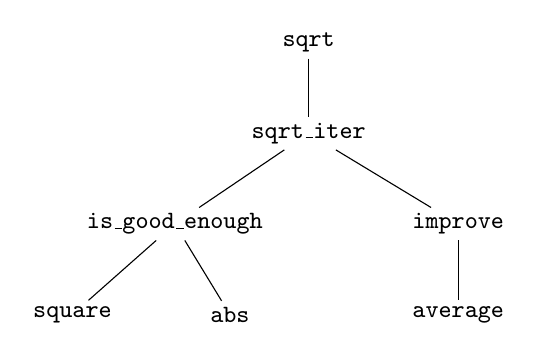
\begin{tikzpicture}[
  x = 1cm, y = 1.15cm,
  every node/.style = {font=\ttfamily\small, inner sep=2pt},
  edge/.style = {draw, thin},
]

\node (sqrt)   at ( 0.0,  0.0) {sqrt};
\node (iter)   at ( 0.0, -1.0) {sqrt\_iter};
\node (enough) at (-1.7, -2.0) {is\_good\_enough};
\node (impr)   at ( 1.9, -2.0) {improve};
\node (sq)     at (-3.0, -3.0) {square};
\node (abs)    at (-1.0, -3.0) {abs};
\node (avg)    at ( 1.9, -3.0) {average};

\foreach \p/\c in {sqrt/iter, iter/enough, iter/impr,
                   enough/sq, enough/abs, impr/avg}
  \draw[edge] (\p) -- (\c);

\end{tikzpicture}
